\documentclass{beamer}
\usepackage{tikz}
\usetikzlibrary{calc}
\usetikzlibrary{arrows.meta}
\usetikzlibrary{backgrounds,matrix,fadings,calc,positioning,decorations.pathreplacing,decorations.markings,arrows.meta,shapes,shapes.multipart}
\usetikzlibrary{patterns,math,quotes,positioning,angles}
\usetikzlibrary{spy}
\usepackage{pgfplots}
\usepackage{xcolor}
\usepackage{siunitx}
\usepackage{chemfig}
\usepackage{amsmath}
\usepackage[version=4]{mhchem}
\usepackage[utf8]{inputenc}

\usetheme{Berlin}
\usecolortheme{default}

\title[Condensation and Evaporation of Hexane in Nanoporous Alumina Membranes]{Condensation and Evaporation of Hexane in Nanoporous Alumina Membranes}
%\subtitle{}
\author[Hermann Böttcher]{Hermann Böttcher\inst{1} \and Victor Doebele\inst{2} \and Pierre-Etienne Wolf\inst{2} \and Panayotis Sphatis\inst{2} \and Fabien Souris\inst{2}}
\institute{
          \inst{1}University of Constance
          \and
          \inst{2}Institut Néel, Centre national de la recherche scientifique
          }
\date[Constance, 02/10/2018]{02/10/2018}
%\logo{\includegraphics[height=1.5cm]{graphics/logoNEEL.png}}

\begin{document}

  \frame{\maketitle}

  \begin{frame}{Overview}
      \begin{enumerate}
        \item Context
        \item Goals of the internship
        \item Theoretical background
        \item Experimental setup
        \item Conclusions
      \end{enumerate}
  \end{frame}

  \begin{frame}{Context}
    \begin{block}{Grand scheme}
      \begin{itemize}
        \item Condensation and evaporation of fluids in confinement
        \pause

        \item Dependency on
          \begin{itemize}
            \item pore diameter
            \item temperature (relative to the critical temperature)
          \end{itemize}
      \end{itemize}
    \end{block}
    \pause

    \begin{block}{Plan}
      \begin{itemize}
        \item Anodized alumina membranes (AAM)
        \item Test setup using Hexane $\rightarrow$ working at room temperature permits much faster executable experiments
        \item Transfer to \textbf{helium} experiment
      \end{itemize}
    \end{block}
  \end{frame}

  \begin{frame}{Goals}
    \begin{itemize}
      \pause
      \item Improving and \textbf{systemizing} the evaluation of the recorded isotherm data

      \item Performing isotherm measurements on many membranes for \textbf{statistics}
      \pause

      \item Comparing the pore diameters extracted from the volumetric measurements those from scanning electron microscopy (SEM) images
      \pause

      \item Improving the fabrication process to reduce the dispersion
      \pause

      \item Testing the efficiency of the ALD process as a means to reduce the pore diameters
    \end{itemize}
  \end{frame}

  \begin{frame}{Condensation in a cylindrical open pore}
    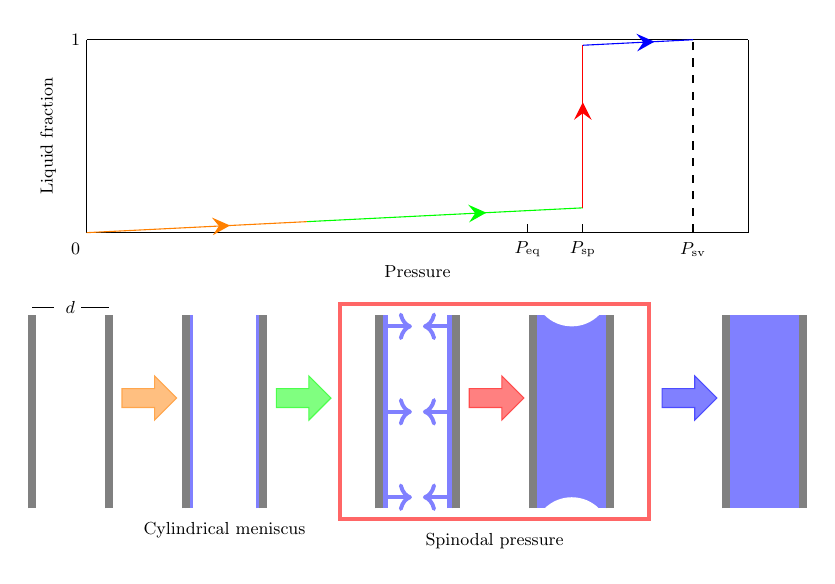
\begin{tikzpicture}[scale=0.7, transform shape,
                          every node/.style = {font = \small},
                          pore/.style = {line width = 0.1cm, color = gray},
                          film/.style = {line width = 0.1cm, color = blue!50},
                          thick_film/.style = {line width = 0.3cm, color = blue!50},
                          graph_label/.style={color = gray, line width = 0.05cm},
                          pore_collapse/.style = {color = blue!50, line width = 0.07cm, ->},
                          MyArrow/.style={single arrow, draw, minimum width=8mm, minimum height=3mm,
                          inner sep=0mm, single arrow head extend=1mm}]
          \tikzset{fontscale/.style = {font=\relsize{#1}}}
          \tikzset{MyArrow/.style={single arrow, draw, minimum width=8mm, minimum height=5mm, inner sep=0mm, single arrow head extend=1mm}}
          \pgfdeclarelayer{bg}    % declare background layer
          \pgfdeclarelayer{bbg}    % declare backbackground layer
          \pgfsetlayers{bbg,bg,main}  % set the order of the layers (main is the standard layer)
          \tikzstyle arrowstyle=[scale=2]
          \tikzstyle directed=[postaction={decorate,decoration={markings,
              mark=at position .65 with {\arrow[arrowstyle]{stealth}}}}]
          \begin{scope}
              \foreach \Xcoor in {0, 1.4, 2.8, 4.2, 6.3, 7.7, 9.1, 10.5, 12.6, 14}
              \draw[pore] (\Xcoor,0) -- (\Xcoor,3.5);
              \draw (0.4,3.65) -- (0,3.65);
              \draw (0.9,3.65) -- (1.4,3.65);
              \node at (0.7,3.65) {$d$};
              \node[draw = orange!70, fill = orange!50, MyArrow] at (2.05, 2) {\phantom{arrow}};
              \node[draw = green!70, fill = green!50, MyArrow] at (4.85, 2) {\phantom{arrow}};
              \node[draw = red!70, fill = red!50, MyArrow] at (8.35, 2) {\phantom{arrow}};
              \node[draw = blue!70, fill = blue!50, MyArrow] at (11.85, 2) {\phantom{arrow}};
              %
              \draw[color = red!60, line width = 0.05cm] (5.6,-0.2) -- (11.2,-0.2) -- (11.2,3.7) -- (5.6,3.7) -- cycle;
              \node at (8.4,-0.6) {Spinodal pressure};
              \node at (3.5,-0.4) {Cylindrical meniscus};
              \begin{pgfonlayer}{bg}    % select the background layer
                  %filmed pore
                  \draw[film] (2.85,0) -- (2.85,3.5);
                  \draw[film] (4.15,0) -- (4.15,3.5);
                  %filmed pore
                  \draw[film] (6.39,0) -- (6.39,3.5);
                  \draw[film] (7.61,0) -- (7.61,3.5);
                  \draw[color = blue!50, ->, line width = 0.5mm] (6.3,0.2) -- (6.9,0.2);
                  \draw[color = blue!50, ->, line width = 0.5mm] (7.7,0.2) -- (7.1,0.2);
                  \draw[color = blue!50, ->, line width = 0.5mm] (6.3,1.75) -- (6.9,1.75);
                  \draw[color = blue!50, ->, line width = 0.5mm] (7.7,1.75) -- (7.1,1.75);
                  \draw[color = blue!50, ->, line width = 0.5mm] (6.3,3.3) -- (6.9,3.3);
                  \draw[color = blue!50, ->, line width = 0.5mm] (7.7,3.3) -- (7.1,3.3);
                  %full pore with menisci
                  \fill[blue!50] (9.1,0) -- (9.1,3.5)  -- (10.5,3.5) -- (10.5,0) -- cycle ;
                  \path [draw = none, fill = white](9.1,4) arc[start angle = -180, end angle = 0, radius=0.7];
                  \path [draw = none, fill = white](9.1,-0.5) arc[start angle = 180, end angle = 0, radius=0.7];
                  %full pore
                  \fill[blue!50] (12.6,0) -- (12.6,3.5)  -- (14,3.5) -- (14,0) -- cycle ;
              \end{pgfonlayer}
          \end{scope}
          \begin{scope}[xshift=1cm,yshift=5cm]
              \draw (0,0) -- (0,3.5);
              \draw (12,0) -- (12,3.5);
              \node[rotate=90] at (-0.7,1.75) {Liquid fraction};
              \draw (0,0) -- (12,0);
              \draw (0,3.5) -- (12,3.5);
              \node at (6,-0.7) {Pressure};
              %yellow
              \draw[color = orange, directed] (0,0) -- (4,0.2);
              %green
              \draw[color = green, directed] (4,0.2) -- (9,0.45);
              %red
              \draw[color = red, directed] (9,0.45) -- (9,3.40);
              %blue
              \draw[color = blue, directed] (9,3.4) -- (11,3.5);
              %DASHED
              \draw[dashed] (11,0) -- (11,3.5);  %psat
              \draw[dashed] (9,0) -- (9,0.3);  %psp
              \draw[dashed] (8,0) -- (8,0.15);  %peq
              %labels
              \node at (-0.2,-0.3) {$0$};
              \node at (-0.2,3.5) {$1$};
              \node at (11,-0.3) {$P_\mathrm{sv}$};
              \node at (8,-0.3) {$P_\mathrm{eq}$};
              \node at (9,-0.3) {$P_\mathrm{sp}$};
          \end{scope}
    \end{tikzpicture}
  \end{frame}

  \begin{frame}{Evaporation in a cylindrical open pore}
    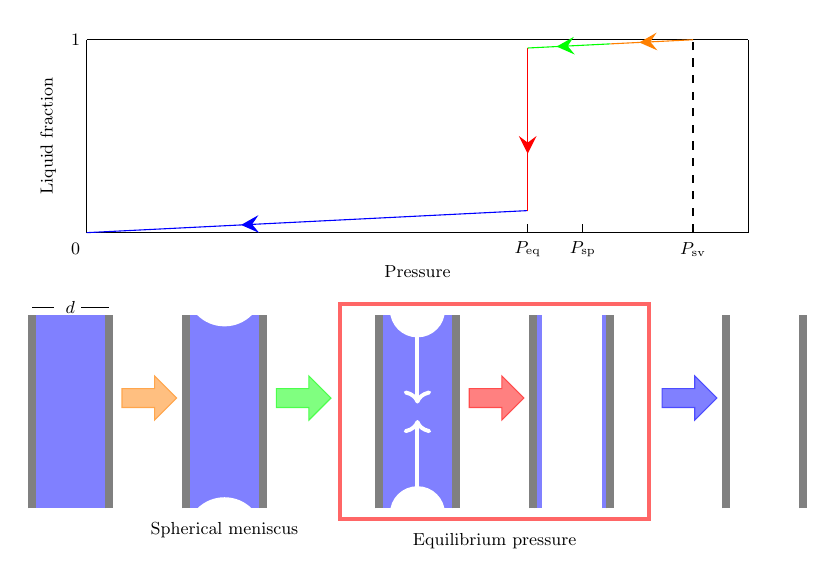
\begin{tikzpicture}[scale=0.7, transform shape,
                            every node/.style = {font = \small},
                            pore/.style = {line width = 0.1cm, color = gray},
                            film/.style = {line width = 0.1cm, color = blue!50},
                            thick_film/.style = {line width = 0.3cm, color = blue!50},
                            graph_label/.style={color = gray, line width = 0.05cm},
                            pore_collapse/.style = {color = blue!50, line width = 0.07cm, ->},
                            MyArrow/.style={single arrow, draw, minimum width=8mm, minimum height=3mm,
                            inner sep=0mm, single arrow head extend=1mm}]
            \tikzset{fontscale/.style = {font=\relsize{#1}}}
            \tikzset{MyArrow/.style={single arrow, draw, minimum width=8mm, minimum height=5mm, inner sep=0mm, single arrow head extend=1mm}}
            \pgfdeclarelayer{bg}    % declare background layer
            \pgfdeclarelayer{bbg}    % declare backbackground layer
            \pgfsetlayers{bbg,bg,main}  % set the order of the layers (main is the standard layer)
            \tikzstyle arrowstyle=[scale=2]
            \tikzstyle directed=[postaction={decorate,decoration={markings,
                mark=at position .65 with {\arrow[arrowstyle]{stealth}}}}]
            \begin{scope}
                \foreach \Xcoor in {0, 1.4, 2.8, 4.2, 6.3, 7.7, 9.1, 10.5, 12.6, 14}
                \draw[pore] (\Xcoor,0) -- (\Xcoor,3.5);
                \draw (0.4,3.65) -- (0,3.65);
                \draw (0.9,3.65) -- (1.4,3.65);
                \node at (0.7,3.65) {$d$};
                \node[draw = orange!70, fill = orange!50, MyArrow] at (2.05, 2) {\phantom{arrow}};
                \node[draw = green!70, fill = green!50, MyArrow] at (4.85, 2) {\phantom{arrow}};
                \node[draw = red!70, fill = red!50, MyArrow] at (8.35, 2) {\phantom{arrow}};
                \node[draw = blue!70, fill = blue!50, MyArrow] at (11.85, 2) {\phantom{arrow}};
                %
                \draw[color = red!60, line width = 0.05cm] (5.6,-0.2) -- (11.2,-0.2) -- (11.2,3.7) -- (5.6,3.7) -- cycle;
                \node at (8.4,-0.6) {Equilibrium pressure};
                \node at (3.5,-0.4) {Spherical meniscus};
                \begin{pgfonlayer}{bg}    % select the background layer
                    %full pore
                    \fill[blue!50] (0,0) -- (0,3.5)  -- (1.4,3.5) -- (1.4,0) -- cycle ;
                    %full pore with menisci
                    \fill[blue!50] (2.8,0) -- (2.8,3.5)  -- (4.2,3.5) -- (4.2,0) -- cycle ;
                    \path [draw = none, fill = white](2.8,4) arc[start angle = -180, end angle = 0, radius=0.7];
                    \path [draw = none, fill = white](2.8,-0.5) arc[start angle = 180, end angle = 0, radius=0.7];
                    %emptying
                    \fill[blue!50] (6.3,0) -- (6.3,3.5)  -- (7.7,3.5) -- (7.7,0) -- cycle ;
                    \path [draw = none, fill = white](6.5,3.6) arc[start angle = -180, end angle = 0, radius=0.5];
                    \path [draw = none, fill = white](6.5,-0.1) arc[start angle = 180, end angle = 0, radius=0.5];
                    \draw[color = white, ->, line width = 0.5mm] (7,0.2) -- (7,1.6);
                    \draw[color = white, ->, line width = 0.5mm] (7,3.8) -- (7,1.9);
                    %filmed pore
                    \draw[film] (9.18,0) -- (9.18,3.5);
                    \draw[film] (10.42,0) -- (10.42,3.5);
                \end{pgfonlayer}
            \end{scope}
            \begin{scope}[xshift=1cm,yshift=5cm]
                \draw (0,0) -- (0,3.5);
                \draw (12,0) -- (12,3.5);
                \node[rotate=90] at (-0.7,1.75) {Liquid fraction};
                \draw (0,0) -- (12,0);
                \draw (0,3.5) -- (12,3.5);
                \node at (6,-0.7) {Pressure};
                %blue
                \draw[color = blue, directed] (8,0.40) -- (0,0);
                %red
                \draw[color = red, directed] (8,3.35) -- (8,0.40);
                %green
                \draw[color = green, directed] (9.5,3.425) -- (8,3.35);
                %orange
                \draw[color = orange, directed] (11,3.5) -- (9.5,3.425);
                %DASHED
                \draw[dashed] (11,0) -- (11,3.5);  %psat
                \draw[dashed] (8,0) -- (8,0.3);  %peq
                \draw[dashed] (9,0) -- (9,0.15);  %psp
                %labels
                \node at (-0.2,-0.3) {$0$};
                \node at (-0.2,3.5) {$1$};
                \node at (11,-0.3) {$P_\mathrm{sv}$};
                \node at (8,-0.3) {$P_\mathrm{eq}$};
                \node at (9,-0.3) {$P_\mathrm{sp}$};
            \end{scope}
    \end{tikzpicture}
  \end{frame}

  \begin{frame}{Condensation and evaporation in a cylindrical open pore}
    \begin{columns}[onlytextwidth, T]
      \column{\dimexpr\linewidth / 3}
        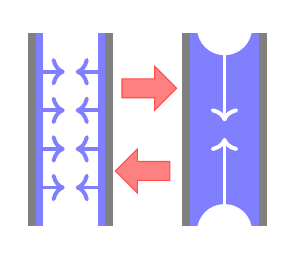
\begin{tikzpicture}[scale=0.7, transform shape,
                              every node/.style = {font = \small},
                              pore/.style = {line width = 0.1cm, color = gray},
                              film/.style = {line width = 0.1cm, color = blue!50},
                              thick_film/.style = {line width = 0.3cm, color = blue!50},
                              graph_label/.style={color = gray, line width = 0.05cm},
                              pore_collapse/.style = {color = blue!50, line width = 0.07cm, ->},
                              MyArrow/.style={single arrow, draw, minimum width=8mm, minimum height=3mm,
                              inner sep=0mm, single arrow head extend=1mm}]
              \tikzset{fontscale/.style = {font=\relsize{#1}}}
              \tikzset{MyArrow/.style={single arrow, draw, minimum width=8mm, minimum height=5mm, inner sep=0mm, single arrow head extend=1mm}}
              \pgfdeclarelayer{bg}    % declare background layer
              \pgfdeclarelayer{bbg}    % declare backbackground layer
              \pgfsetlayers{bbg,bg,main}  % set the order of the layers (main is the standard layer)
              \tikzstyle arrowstyle=[scale=2]
              \tikzstyle directed=[postaction={decorate,decoration={markings,
                  mark=at position .65 with {\arrow[arrowstyle]{stealth}}}}]
              \begin{scope}
                  \foreach \Xcoor in {0, 2.8}{
                  \draw[pore] (\Xcoor,3.5) -- (\Xcoor,0);
                  \draw[pore] (\Xcoor + 1.4,0) -- (\Xcoor + 1.4,3.5);}
                  \node[draw = red!70, fill = red!50, MyArrow] at (2.05, 2.5) {\phantom{arrow}};
                  \node[draw = red!70, fill = red!50, MyArrow, rotate = 180] at (2.1, 1) {\phantom{arrow}};
                  \begin{pgfonlayer}{bg}
                      \fill[blue!50] (2.8,0) -- (2.8,3.5)  -- (4.2,3.5) -- (4.2,0) -- cycle ;
                      \fill[blue!50] (0,0) -- (0,3.5)  -- (0.2,3.5) -- (0.2,0) -- cycle;
                      \fill[blue!50] (1.4,0)--(1.4,3.5)--(1.2,3.5)--(1.2,0)--cycle;
                      \path [draw = none, fill = white](3,3.6) arc[start angle = -180, end angle = 0, radius=0.5];
                      \path [draw = none, fill = white](3,-0.1) arc[start angle = +180, end angle = 0, radius=0.5];
                      \foreach \Y in {0.7,1.4,2.1,2.8}{
                          \draw[color=blue!50, ->, line width=0.5mm] (0,\Y) -- (0.6,\Y);
                          \draw[color=blue!50, ->, line width=0.5mm] (1.4,\Y) -- (0.8,\Y);
                          }
                      \draw[color = white, ->, line width = 0.5mm] (3.5,3.3) -- (3.5,1.9);
                      \draw[color = white, ->, line width = 0.5mm] (3.5,0.2) -- (3.5,1.6);
                  \end{pgfonlayer}
              \end{scope}
        \end{tikzpicture}
      \column{\dimexpr\linewidth / 3 * 2}
        \begin{block}{Open cylindrical pore}
          Condensation at spinodal pressure and \\
          evaporation at equilibrium pressure \\
          yield a \textbf{hysteresis.}
        \end{block}
    \end{columns}
        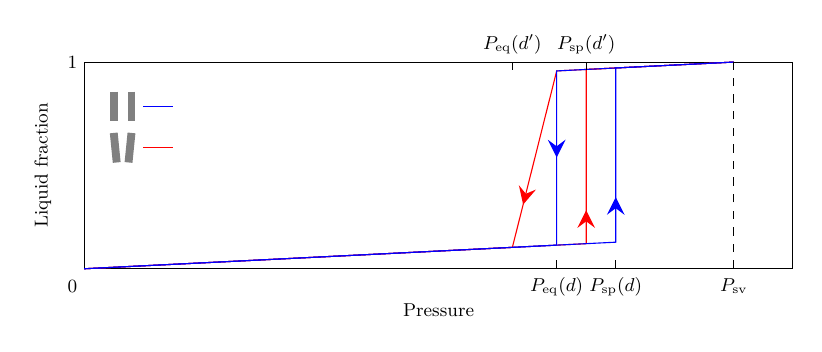
\begin{tikzpicture}[scale=0.75, transform shape, every node/.style = {font = \small},
                          pore/.style = {line width = 0.1cm, color = gray},
                          film/.style = {line width = 0.1cm, color = blue!50},
                          thick_film/.style = {line width = 0.3cm, color = blue!50},
                          graph_label/.style={color = gray, line width = 0.05cm},
                          pore_collapse/.style = {color = blue!50, line width = 0.07cm, ->},
                          MyArrow/.style={single arrow, draw, minimum width=8mm, minimum height=3mm, inner sep=0mm, single arrow head extend=1mm}]
          \tikzset{fontscale/.style = {font=\relsize{#1}}}
          \tikzset{MyArrow/.style={single arrow, draw, minimum width=8mm, minimum height=5mm, inner sep=0mm, single arrow head extend=1mm}}
          \pgfdeclarelayer{bg}    % declare background layer
          \pgfdeclarelayer{bbg}    % declare backbackground layer
          \pgfsetlayers{bbg,bg,main}  % set the order of the layers (main is the standard layer)
          \tikzstyle arrowstyle=[scale=2]
          \begin{scope}
              \draw (0,0) -- (0,3.5);
              \draw (12,0) -- (12,3.5);
              \node[rotate=90] at (-0.7,1.75) {Liquid fraction};
              \draw (0,0) -- (12,0);
              \draw (0,3.5) -- (12,3.5);
              \node at (6,-0.7) {Pressure};
              %cond funnel
              \draw[color = red, postaction={decorate,decoration={markings,
              mark=at position .65 with {\arrow[arrowstyle]{stealth}}}}] (0,0) -- (8.5,0.425) -- (8.5,3.375) -- (11,3.5);
              %evap funnel
              \draw[color = red, postaction={decorate,decoration={markings,
              mark=at position .4 with {\arrow[arrowstyle]{stealth}}}}] (11,3.5) -- (8,3.35) -- (7.25,0.3625) -- (0,0);
              %cond straight
              \draw[color = blue, postaction={decorate,decoration={markings,
              mark=at position .70 with {\arrow[arrowstyle]{stealth}}}}] (0,0) -- (9,0.45) -- (9,3.40) -- (11,3.5);
              %evap straight
              \draw[color = blue, postaction={decorate,decoration={markings,
              mark=at position .32 with {\arrow[arrowstyle]{stealth}}}}] (11,3.5) -- (8,3.35) -- (8,0.4) -- (8,0.40) -- (0,0);
              %DASHED
              \draw[dashed] (11,0) -- (11,3.5);  %psat
              \draw[dashed] (9,0) -- (9,0.15);  %psp
              \draw[dashed] (8,0) -- (8,0.15);  %peq
              \draw[dashed] (8.5,3.5) -- (8.5,3.35);  %psp
              \draw[dashed] (7.25,3.5) -- (7.25,3.35);  %peq
              %labels
              %labels
              \node at (-0.2,-0.3) {$0$};
              \node at (-0.2,3.5) {$1$};
              \node at (11,-0.3) {$P_\mathrm{sv}$};
              \node at (8,-0.3) {$P_\mathrm{eq}(d)$};
              \node at (9,-0.3) {$P_\mathrm{sp}(d)$};
              \node at (7.25,3.8) {$P_\mathrm{eq}(d')$};
              \node at (8.5,3.8) {$P_\mathrm{sp}(d')$};
              \draw[color=gray, line width=1mm] (0.5,3) -- (0.5,2.5);
              \draw[color=gray, line width=1mm] (0.8,3) -- (0.8,2.5);
              \draw[color=blue] (1,2.75) -- (1.5,2.75);
              \draw[color=gray, line width=1mm] (0.5,2.3) -- (0.55,1.8);
              \draw[color=gray, line width=1mm] (0.8,2.3) -- (0.75,1.8);
              \draw[color=red] (1,2.05) -- (1.5,2.05);
          \end{scope}
        \end{tikzpicture}
  \end{frame}

  \begin{frame}{Condensation and evaporation in a cylindrical open pore}
    \begin{columns}[onlytextwidth, T]
      \column{\dimexpr\linewidth / 3}
          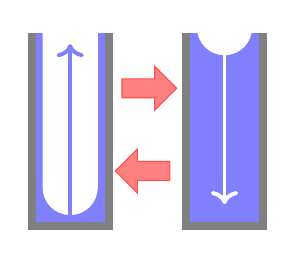
\begin{tikzpicture}[scale=0.7, transform shape, every node/.style = {font = \small},
                              pore/.style = {line width = 0.1cm, color = gray},
                              film/.style = {line width = 0.1cm, color = blue!50},
                              thick_film/.style = {line width = 0.3cm, color = blue!50},
                              graph_label/.style={color = gray, line width = 0.05cm},
                              pore_collapse/.style = {color = blue!50, line width = 0.07cm, ->},
                              MyArrow/.style={single arrow, draw, minimum width=8mm, minimum height=3mm,
                              inner sep=0mm, single arrow head extend=1mm}]
              \tikzset{fontscale/.style = {font=\relsize{#1}}}
              \tikzset{MyArrow/.style={single arrow, draw, minimum width=8mm, minimum height=5mm, inner sep=0mm, single arrow head extend=1mm}}
              \pgfdeclarelayer{bg}    % declare background layer
              \pgfdeclarelayer{bbg}    % declare backbackground layer
              \pgfsetlayers{bbg,bg,main}  % set the order of the layers (main is the standard layer)
              \tikzstyle arrowstyle=[scale=2]
              \tikzstyle directed=[postaction={decorate,decoration={markings,
                  mark=at position .65 with {\arrow[arrowstyle]{stealth}}}}]
              \begin{scope}
                  \foreach \Xcoor in {0, 2.8}
                  \draw[pore] (\Xcoor,3.5) -- (\Xcoor,0) -- (\Xcoor + 1.4,0) -- (\Xcoor + 1.4,3.5);
                  \node[draw = red!70, fill = red!50, MyArrow] at (2.05, 2.5) {\phantom{arrow}};
                  \node[draw = red!70, fill = red!50, MyArrow, rotate = 180] at (2.1, 1) {\phantom{arrow}};
                  \begin{pgfonlayer}{bg}
                      \fill[blue!50] (2.8,0) -- (2.8,3.5)  -- (4.2,3.5) -- (4.2,0) -- cycle ;
                      \fill[blue!50] (0,0) -- (0,3.5)  -- (1.4,3.5) -- (1.4,0) -- cycle ;
                      \path [draw = none, fill = white](3,3.6) arc[start angle = -180, end angle = 0, radius=0.5];
                      \fill[white] (1.2,3.55) -- (0.2,3.55) -- (0.2,0.7) arc[start angle = -180, end angle = 0, radius=0.5] -- cycle;
                      \draw[color = blue!50, ->, line width = 0.5mm] (0.7,0.2) -- (0.7,3.3);
                      \draw[color = white, ->, line width = 0.5mm] (3.5,3.3) -- (3.5,0.4);
                  \end{pgfonlayer}
              \end{scope}
          \end{tikzpicture}
      \column{\dimexpr\linewidth / 3 * 2}
        \begin{block}{Closed cylindrical pore}
          Condensation at equilibrium pressure and \\
          evaporation at equilibrium pressure \\
          leads to \textbf{disappearance of the hysteresis.}
        \end{block}
    \end{columns}
    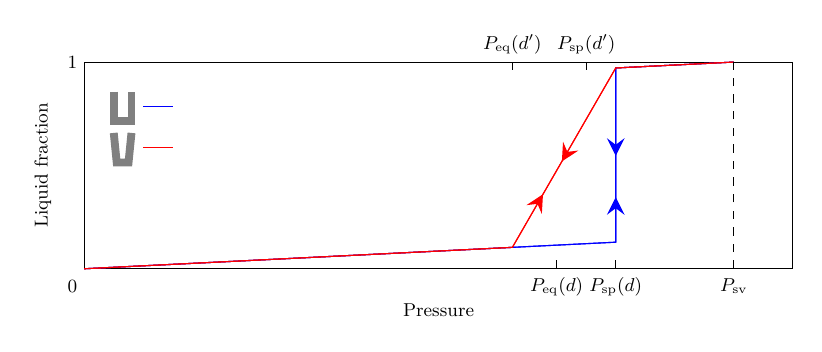
\begin{tikzpicture}[scale=0.75, transform shape, every node/.style = {font = \small},
                        pore/.style = {line width = 0.1cm, color = gray},
                        film/.style = {line width = 0.1cm, color = blue!50},
                        thick_film/.style = {line width = 0.3cm, color = blue!50},
                        graph_label/.style={color = gray, line width = 0.05cm},
                        pore_collapse/.style = {color = blue!50, line width = 0.07cm, ->},
                        MyArrow/.style={single arrow, draw, minimum width=8mm, minimum height=5mm,
                        inner sep=0mm, single arrow head extend=1mm}]
        \pgfdeclarelayer{bg}    % declare background layer
        \pgfdeclarelayer{bbg}    % declare backbackground layer
        \pgfsetlayers{bbg,bg,main}  % set the order of the layers (main is the standard layer)
        \tikzset{fontscale/.style = {font=\relsize{#1}}}
        \tikzset{MyArrow/.style={single arrow, draw, minimum width=8mm, minimum height=5mm, inner sep=0mm, single arrow head extend=1mm}}
        \tikzstyle arrowstyle=[scale=2]
        \tikzstyle directed=[postaction={decorate,decoration={markings,
            mark=at position .65 with {\arrow[arrowstyle]{stealth}}}}]
        \begin{scope}
            \draw (0,0) -- (0,3.5);
            \draw (12,0) -- (12,3.5);
            \node[rotate=90] at (-0.7,1.75) {Liquid fraction};
            \draw (0,0) -- (12,0);
            \draw (0,3.5) -- (12,3.5);
            \node at (6,-0.7) {Pressure};
            %straight evap
            \draw[color = blue, postaction={decorate,decoration={markings,
            mark=at position .25 with {\arrow[arrowstyle]{stealth}}}}] (11,3.5) -- (9,3.4) -- (9,0.45) -- (0,0);
            %straight cond
            \draw[color = blue, postaction={decorate,decoration={markings,
            mark=at position .7 with {\arrow[arrowstyle]{stealth}}}}] (0,0) -- (9,0.45) -- (9,3.4) -- (11,3.5);
            %funnelled 1 cond
            \draw[color = red, postaction={decorate,decoration={markings,
            mark=at position .65 with {\arrow[arrowstyle]{stealth}}}}] (0,0) -- (7.25,0.3625) -- (9,3.4) -- (11,3.5);
            %funnelled 1 evap
            \draw[color = red, postaction={decorate,decoration={markings,
            mark=at position .3 with {\arrow[arrowstyle]{stealth}}}}] (11,3.5) -- (9,3.4) -- (7.25,0.3625) -- (0,0);
            %DASHED
            \draw[dashed] (11,0) -- (11,3.5);  %psat
            \draw[dashed] (9,0) -- (9,0.15);  %psp
            \draw[dashed] (8,0) -- (8,0.15);  %peq
            \draw[dashed] (8.5,3.5) -- (8.5,3.35);  %psp
            \draw[dashed] (7.25,3.5) -- (7.25,3.35);  %peq
            %labels
            \node at (-0.2,-0.3) {$0$};
            \node at (-0.2,3.5) {$1$};
            \node at (11,-0.3) {$P_\mathrm{sv}$};
            \node at (8,-0.3) {$P_\mathrm{eq}(d)$};
            \node at (9,-0.3) {$P_\mathrm{sp}(d)$};
            \node at (7.25,3.8) {$P_\mathrm{eq}(d')$};
            \node at (8.5,3.8) {$P_\mathrm{sp}(d')$};
            \draw[color=gray, line width=1mm] (0.5,3) -- (0.5,2.5) -- (0.8,2.5) -- (0.8,3);
            \draw[color=blue] (1,2.75) -- (1.5,2.75);
            \draw[color=gray, line width=1mm] (0.5,2.3) -- (0.55,1.8) -- (0.75,1.8) -- (0.8,2.3);
            \draw[color=red] (1,2.05) -- (1.5,2.05);
        \end{scope}
    \end{tikzpicture}
  \end{frame}

  \begin{frame}{Membrane production}
         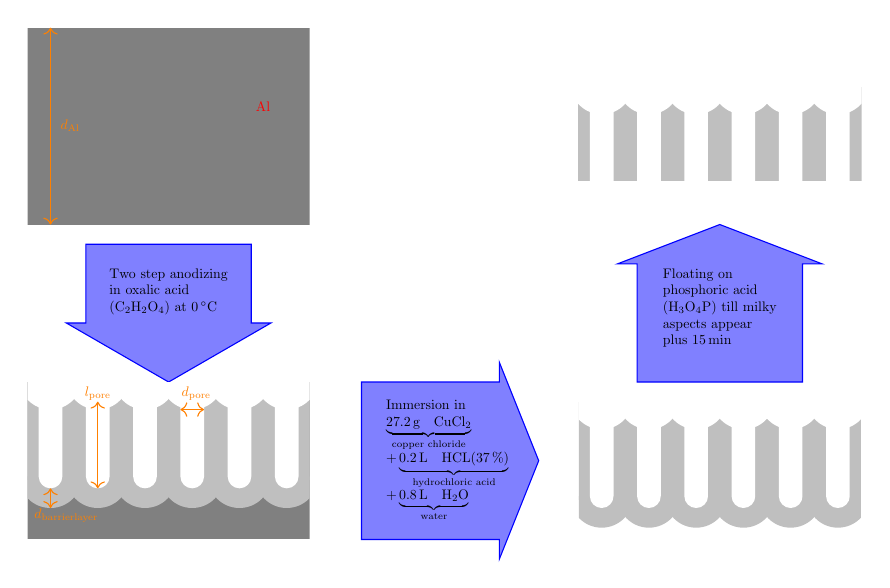
\begin{tikzpicture}[scale=0.5, transform shape,
                             MyArrow/.style={single arrow, draw, minimum width=16mm, minimum height=12mm,
                             inner sep=0mm, single arrow head extend=2mm}]
             %\tikzset{fontscale/.style = {font=\relsize{#1}}}
             \tikzset{MyArrow/.style={single arrow, draw, minimum width=16mm, minimum height=10mm, inner sep=0mm, single arrow head extend=.8mm}}
           \begin{scope}
              \def\l{7.2};
              \def\h{5};
              \def\d{0.8};
              %\node[draw = blue!70, fill = blue!50, MyArrow, rotate=270] at (2.6, -2) {\phantom{arrow}};
              %\node[anchor=west, align=left] at (3.6,-2) {Two step anodizing\\ in oxalic acid\\ (\ce{C2H2O4}) at $\SI{0}{\celsius}$};
              %\draw[fill=blue!50, color=blue] (3.6,-3)--(2.6,-2)--(3.1,-2)--(3.1,-1)--(4.2,-1)--(4.2,-2)--(4.6,-2)--(3.6,-3);
              \fill[color=blue!50, draw=blue] (1.5,-.5)--(5.7,-.5)--(5.7,-2.5)--(6.2,-2.5)--(3.6,-4)--(1,-2.5)--(1.5,-2.5)--cycle;
              \node[anchor=north, align=left] at (3.6,-1) {Two step anodizing\\ in oxalic acid\\ (\ce{C2H2O4}) at $\SI{0}{\celsius}$};
              \clip (0.02,0) rectangle (\l - 0.02,\h);
              \fill[gray] (0,0) rectangle (\l,\h);
              \draw[color=orange,<->] (0.6,0) -- (0.6,\h);
              \node[color=orange] at (1.1,\h/2) {$d_\mathrm{Al}$};
              \node[color=red] at (6,3) {$\ce{Al}$};
           \end{scope}
           \begin{scope}[yshift=-8cm]
               \def\l{7.2};
               \def\h{4};
               \def\d{0.6};
               %\node[draw = blue!70, fill = blue!50, MyArrow] at (11, 2) {\phantom{arrow}};
               %\node[anchor=south, align=left] at (11,3) {Immersion in\\ $\underbrace{\SI{27,2}{\gram}\quad\ce{CuCl2}}_{\text{copper chloride}}$\\ $ + \underbrace{\SI{0,2}{\l}\quad\ce{HCL}(\SI{37}{\percent})}_{\text{hydrochloric acid}}$\\ $+ \underbrace{\SI{0,8}{\l}\quad\ce{H2O}}_{\text{water}}$};
               \fill[color=blue!50, draw=blue] (8.5,0)--(8.5,4)--(12,4)--(12,4.5)--(13,2)--(12,-.5)--(12,0)--cycle;
               \node[anchor=west, align=left] at (9,2) {Immersion in\\ $\underbrace{\SI{27,2}{\gram}\quad\ce{CuCl2}}_{\text{copper chloride}}$\\ $ + \underbrace{\SI{0,2}{\l}\quad\ce{HCL}(\SI{37}{\percent})}_{\text{hydrochloric acid}}$\\ $+ \underbrace{\SI{0,8}{\l}\quad\ce{H2O}}_{\text{water}}$};
               \begin{scope}
               \clip (0.02,0) rectangle (\l - 0.02,\h);
               \fill[gray] (0,0) rectangle (\l,\h);
               \fill[lightgray] (0,1.5) rectangle (\l,\h);
               \foreach \i in {1,3,...,11}{
                   \fill[white] (- 4 / 3 * \d + \i * \d, \h + 0.1) arc (180:360:\d / 3 * 4);
                   \fill[lightgray] (- 4 / 3 * \d + \i * \d, \h - 2.5 + 0.1) arc (180:360:\d / 3 * 4);
                   \fill[white] (-0.5 * \d + \i * \d, \h - 2.5 + 0.1) arc (180:360:\d / 2) -- (-0.5 * \d + \i * \d + \d, \h + 0.1) -- (-0.5 * \d + \i * \d, \h + 0.1) -- cycle;}
               \draw[color=orange,<->] (3.9,3.3) -- (4.5,3.3);
               \node[color=orange] at (4.3,3.7) {$d_\mathrm{pore}$};
               \draw[color=orange,<->] (0.6,\h-2.5+0.1-0.3) -- (0.6,\h-2.5+0.1-0.8);
               \node[color=orange] at (1,\h-2.5+0.1-0.8-0.2) {$d_\mathrm{barrier layer}$};
               \draw[color=orange,<->] (1.8,\h-2.5+0.1-0.3) -- (1.8,\h-+0.1-0.4);
               \node[color=orange] at (1.8,\h-0.3) {$l_\mathrm{pore}$};
               \end{scope}
            \end{scope}
            \begin{scope}[yshift=-8cm, xshift=14cm]
                \def\l{7.2};
                \def\h{3.5};
                \def\d{0.6};
                %\node[draw = blue!70, fill = blue!50, MyArrow, rotate=90] at (4.6, 6) {\phantom{arrow}};
                %\node[anchor=east, align=left] at (4.6,6) {Floating on\\ phosphoric acid\\ (\ce{H3O4P})};
                \fill[color=blue!50, draw=blue] (1.5,4)--(5.7,4)--(5.7,7)--(6.2,7)--(3.6,8)--(1,7)--(1.5,7)--cycle;
                \node[anchor=north, align=left] at (3.6,7) {Floating on\\ phosphoric acid\\ (\ce{H3O4P}) till milky\\ aspects appear\\ plus $\SI{15}{\minute}$};
                \begin{scope}
                \clip (0.02,0) rectangle (\l - 0.02,\h);
                %\fill[gray] (0,0) rectangle (\l,\h);
                \fill[lightgray] (0,1) rectangle (\l,\h);
                \foreach \i in {1,3,...,11}{
                    \fill[white] (- 4 / 3 * \d + \i * \d, \h + 0.1) arc (180:360:\d / 3 * 4);
                    \fill[lightgray] (- 4 / 3 * \d + \i * \d, \h - 2.5 + 0.1) arc (180:360:\d / 3 * 4);
                    \fill[white] (-0.5 * \d + \i * \d, \h - 2.5 + 0.1) arc (180:360:\d / 2) -- (-0.5 * \d + \i * \d + \d, \h + 0.1) -- (-0.5 * \d + \i * \d, \h + 0.1) -- cycle;}
                \end{scope}
            \end{scope}
            \begin{scope}[xshift=14cm]
                \def\l{7.2};
                \def\h{3.5};
                \def\d{0.6};
                \begin{scope}
                \clip (0,0) rectangle (\l,\h);
                \fill[lightgray] (0,1.1) rectangle (\l,\h);
                \foreach \i in {1,3,...,11}{
                    \fill[white] (- 4 / 3 * \d + \i * \d, \h + 0.1) arc (180:360:\d / 3 * 4);
                    \fill[white] (-0.5 * \d + \i * \d, \h - 2.5 + 0.1) arc (180:360:\d / 2) -- (-0.5 * \d + \i * \d + \d, \h + 0.1) -- (-0.5 * \d + \i * \d, \h + 0.1) -- cycle;}
                \end{scope}
            \end{scope}
         \end{tikzpicture}
  \end{frame}

  \begin{frame}{Alumina membranes - funnellization}
    \begin{columns}[onlytextwidth, T]
      \column{\dimexpr\linewidth / 3 * 2}

        \includegraphics[width=\linewidth]{images/membranes.pdf}
        \pause

        \begin{columns}[onlytextwidth, T]
          \column{\dimexpr\linewidth / 2}
            \includegraphics[width=\linewidth]{images/295c__al_side.jpg}
          \column{\dimexpr\linewidth / 2}
            \includegraphics[width=\linewidth]{images/295c_sol_side.jpg}
        \end{columns}
        \pause

        \column{\dimexpr\linewidth / 3}
        \begin{block}{Funnellization}
          Funnellization suspected due to different pore diameters on top\\ and bottom side.
        \end{block}
        \begin{tikzpicture}[scale=0.6, shape transform]
          \draw[color=blue!80, line width=2mm] (0,0)--(2,0)--(1,3)--(0,3);
          \draw[color=blue!80, line width=2mm] (6,0)--(4,0)--(5,3)--(6,3);
        \end{tikzpicture}
    \end{columns}
  \end{frame}



  \begin{frame}{Alumina membranes - pore size distribution}
    \begin{columns}[onlytextwidth, T]
      \column{\dimexpr\linewidth / 3 * 2}
        \includegraphics[width=\linewidth]{images/AAM_295_PO_30_hist.png}
      \column{\dimexpr\linewidth / 3}
        \begin{block}{Pore size distribution}
          SEM analysis shows pore size distribution on a given membrane.
        \end{block}
    \end{columns}
  \end{frame}



  \begin{frame}{Alumina membranes - corrugations}
    \begin{columns}[onlytextwidth, T]
      \column{\dimexpr\linewidth / 2}
        \begin{tikzpicture}[scale=0.6, transform shape]
            \def\PrelMin{.86}
            \def\PrelMax{1}
            \def\TransMin{1e-8}
            \def\TransMax{10}
            \def\LfMin{0}
            \def\LfMax{1}
            %
            \begin{axis}[
              /tikz/line join=bevel,
              %width=0.8*\textwidth,
              %height=0.5*\textwidth,
              grid,
              %axis y line*=left,
              legend style={at={(0,1)}, legend columns=1, anchor=north west},
              every axis plot,
              line width = 1pt,
              %	minor x tick num= ,
              %	minor y tick num= ,
              xmin = \PrelMin, xmax = \PrelMax,
              ymin = \LfMin, ymax = \LfMax,
              xlabel = {Relative pressure $P_\mathrm{rel}$},
              ylabel = {Liquid fraction $LF$},
              ytick = {0,0.25,0.50,0.75,1},
              title=Closed pores,
              ]
              % Add plots
              \addplot[mark=none, color=red] table [x=Prel,y=liquid_fraction]{tikz/graphs/296_op_cp_comparison/296b_cp_cond_1.txt};
              \addlegendentry{$LF_\mathrm{cond}^\mathrm{296b}$}
              \addplot[mark=none, color=blue] table [x=Prel,y=liquid_fraction]{tikz/graphs/296_op_cp_comparison/296b_cp_evap_1.txt};
              \addlegendentry{$LF_\mathrm{evap}^\mathrm{296b}$}
            \end{axis}
        \end{tikzpicture}
        \pause

      \column{\dimexpr\linewidth / 2}
        \begin{block}{Corrugations}
          The appearance of the hysteresis is assumed to be due to \textbf{intra pore corrugations}.
        \end{block}
        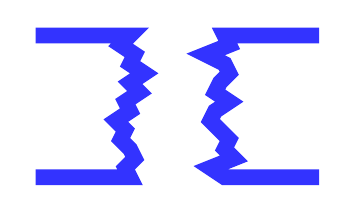
\begin{tikzpicture}[scale=0.6, transform shape]
          \draw[color=blue!80, line width=2mm] (0,0)--(2,0)--(1.9,0.2)--(2.1,0.4)--(2,0.6)--(1.8,0.8)--(1.9,1)--(1.7,1.2)--(2,1.4)--(1.9,1.6)--(2.2,1.8)--(2,2)--(2.3,2.2)--(2,2.4)--(2.1,2.6)--(1.8,2.8)--(2,3)--(0,3);
            \draw[color=blue!80, line width=2mm] (6,0)--(4,0)--(3.7,0.2)--(4.2,0.4)--(4,0.6)--(4.1,0.8)--(3.9,1)--(3.7,1.2)--(3.8,1.4)--(4.1,1.6)--(3.8,1.8)--(3.9,2)--(4.1,2.2)--(4,2.4)--(3.6,2.6)--(4.1,2.8)--(4,3)--(6,3);
        \end{tikzpicture}
    \end{columns}
  \end{frame}



  \begin{frame}{Alumina membrane defects}
    \begin{block}{Isotherms are affected by}
      \begin{itemize}
        \item Pore size distribution
        \item Funnellization
        \item Corrugations
      \end{itemize}
    \end{block}
    \pause

    \begin{alertblock}{Problem}
      No simple ways to characterize these defects!\\
      SEM images only give an impression of the surfaces of the membrane (factor between pore diameter and pore length is 1000!).\\
      $\quad\rightarrow$ Need of \textbf{monodisperse membranes}
    \end{alertblock}
  \end{frame}



  \begin{frame}{Final experimental setup}
    \pgfdeclarelayer{bg}    % declare background layer
    \pgfdeclarelayer{bbg}    % declare backbackground layer
    \pgfsetlayers{bbg,bg,main}  % set the order of the layers (main is the standard layer)
    \begin{tikzpicture}[scale=0.7, transform shape]
        %objects
        \draw[color=orange!60,line width=1mm,fill = white] decorate[decoration={snake},decorate] {(0,2) -- (2,2)} -- (2,1) -- (0,1) -- (0,2);
        \node at (1,1.5) {$T_\mathrm{res}$};
        \node at (1,0.5) {Reservoir};
        \draw[color=orange!60,line width=1mm] (0,1) rectangle (2,3);

        \begin{scope}[xshift=-1.5cm]
          \draw[color=orange!60,line width=1mm] (4,3) -- (4.5,3.5) -- (4,4) -- cycle;
          \draw[color=blue!60,line width=1mm] (5,4) -- (4.5,3.5) -- (5,3) -- cycle;
          \node at (4.5,2.7) {$V_1$};
          \draw[color=blue!60,line width=1mm] (6,1) -- (7,2) -- (7,1) -- (6,2) -- cycle;
          \node at (6.5,0.7) {$V_2$};
          \draw[color=blue!60,line width=1mm] (8,3) -- (8.5,3.5) -- (8,4) -- cycle;
          \draw[color=green!60,line width=1mm] (9,4) -- (8.5,3.5) -- (9,3) -- cycle;
          \node at (8.5,2.7) {$V_3$};
          \draw[color=blue!60,line width=1mm] (8,6) -- (8.5,5.5) -- (8,5) -- cycle;
          \draw[color=green!60,line width=1mm] (9,6) -- (8.5,5.5) -- (9,5) -- cycle;
          \fill[circle, gray] (8.5,5.5) circle (0.25);
          \draw[color=green!60,line width=1mm] (12,3.5) circle (1);
          \draw[color=green!60,line width=1mm, fill=gray!20] (11.5,3) rectangle (12.5,4);
          \draw[color=blue!60, line width=1mm] (10,1) -- (9,1) -- (9,2) -- (10,2);
          \node at (14,6) {$P_\mathrm{cell}$};
          \draw[rectangle, color = green!60, line width=1mm] (13.5,5.5) rectangle (14.5,6.5);
          \draw[rectangle, color=blue!60, line width=1mm] (4,5) rectangle (5,6);
          \node at (4.5,5.5) {$P_\mathrm{res}$};
          \node at (9.5,0.5) {Void};
          \node at (11,2.5) {Cell};
          \node at (8.5,6.5) {\textsc{Pfeiffer} microvalve};
          \draw (11.75,0) rectangle (12.25,1.5);
          \begin{pgfonlayer}{bg}
            \draw[line width=1pt, color=red] (12,1.5)--(12,3);
            \draw[line width=1pt, color=red] (12,4)--(12,5.75);
          \end{pgfonlayer}
          \node at (13.5,1) {\ce{HeNe} Laser};
          \begin{scope}[yshift=-0.5cm]
            \draw[fill=white] (14.5,2.25) rectangle (16,2.75);
            \node at (15.25,2.5) {Camera};
            \draw (11.75,2.75)--(12.25,2.25)--(12.25,2.75)--(11.75,2.75)--(11.75,2.25)--(11.75,2.25)--(12.25,2.25);
          \end{scope}
          \begin{scope}[yshift=0.5cm]
            \draw (11.75,5.25) rectangle (12.25,5.75);
            \node at (12,6) {Photodiode};
            \draw[fill=white] (14.5,4.25) rectangle (16,4.75);
            \node at (15.25,4.5) {LED};
            \draw (11.75,4.25)--(12.25,4.75)--(11.75,4.75)--(11.75,4.25)--(12.25,4.25)--(12.25,4.75);
          \end{scope}
          \begin{pgfonlayer}{bbg}
            \fill[gray!20] (12,5)--(12.5,4)--(11.5,4)--cycle;
            \fill[gray!20] (12,2)--(12.5,3)--(11.5,3)--cycle;
            \draw[color=gray!20,line width=1mm] (14.5,2)--(12,2);
            \draw[color=gray!20,line width=1mm] (14.5,5)--(12,5);
          \end{pgfonlayer}
        \end{scope}
        %pipes
        \begin{pgfonlayer}{bg}    % select the background layer
            \draw[color=orange!60, line width=1mm] (1,2.5) -- (1,3.5) -- (2.5,3.5);
            \begin{scope}[xshift=-1.5cm]
              \draw[color=blue!60,line width=1mm] (5,3.5) -- (8,3.5);
              \draw[color = green!60, line width=1mm] (9,3.5) -- (11,3.5);
              \draw[color = green!60, line width=1mm] (13,3.5) -- (14,3.5) -- (14,5.5);
              \draw[color=blue!60,line width=1mm] (6.5,1.5) -- (6.5,5.5);
              \draw[color=blue!60,line width=1mm] (7,1.5) -- (9,1.5);
              \draw[color=blue!60,line width=1mm] (8,5.5) -- (5,5.5);
              \draw[color = green!50, line width=1mm] (9,5.5) -- (10,5.5) -- (10,3.5);
            \end{scope}
        \end{pgfonlayer}
        %\begin{pgfonlayer}{bbg}    % select the background layer
        %    \draw[color = green!60, line width=2mm] (8.5,6) -- (8.5,2.5) -- (11,2.5) %-- (11,1) -- (15,1) -- (15,6) -- cycle;
        %\end{pgfonlayer}
        \begin{scope}[xshift=-1.5cm]
          \node at (12,3.5) {$T_\mathrm{cell}$};
        \end{scope}
    \end{tikzpicture}
    \pause

    \begin{alertblock}{Volumetric and optical measurements}
      Volumetric and optical setups work independently.
    \end{alertblock}



  \end{frame}



  \begin{frame}{Data evaluation}

  \end{frame}



  \begin{frame}{Inverse funnelling}

  \end{frame}



  \begin{frame}{Atomic layer deposition}

  \end{frame}



  \begin{frame}{SEM image analysis}
    \includegraphics[width=\linewidth]{images/AAM_295_PO_30 um_Al_26.tif.png}
  \end{frame}


\end{document}
